% Fragment prepared for insertion into the Stokes solver section of
% /Users/tgol0006/uw_folder/UW3_benchmarks/Combined_document.tex.
% It summarises only volume L2 velocity and pressure errors from the
% annulus and spherical-shell benchmark articles.

\subsubsection{Annulus and spherical-shell Stokes benchmarks}

The Cartesian benchmarks provide a useful verification framework for Stokes
flow on simple planar domains. To further assess the robustness of the solver
in geometries relevant to geodynamics, we also consider annulus and
spherical-shell benchmark problems. These benchmarks introduce additional
complexities associated with curved boundaries, radial gravity, non-trivial
pressure distributions, and velocity boundary conditions imposed on
non-planar surfaces. Such configurations are representative of mantle
convection and lithospheric deformation models, and therefore provide a more
stringent test of the finite-element implementation.

Model accuracy is quantified using relative volume \(L_2\)-norm errors for the
velocity and pressure fields. For a numerical solution \(q_h\) and analytical
reference solution \(q^{*}\), the relative error is defined as
\begin{equation}
E_{L_2}^{\mathrm{rel}}(q)
=
\left(
\frac{\int_{\Omega} |q_h-q^{*}|^2 \,\mathrm{d}\Omega}
     {\int_{\Omega} |q^{*}|^2 \,\mathrm{d}\Omega}
\right)^{1/2}.
\end{equation}
This definition is applied to both velocity and pressure. Since the
incompressible Stokes equations determine pressure only up to an additive
constant, the numerical and analytical pressures are compared after removing
their mean values to enforce a common pressure gauge.

\textbf{Benchmark setup}
The annulus benchmarks use analytical Stokes solutions defined in cylindrical
shell geometry. The Thieulot--Puckett annulus benchmark provides a smooth
manufactured solution for incompressible Stokes flow driven by radial gravity,
with tangential velocity conditions imposed on the inner and outer boundaries.
This benchmark is well suited for assessing the optimal convergence behaviour
of mixed finite-element discretisations
\citep{thieulot2018,girault1986femns,boffi2013}. The Kramer annulus benchmark
extends this framework by distinguishing between smooth volumetric forcing and
delta-function forcing applied on an internal circular interface, and by
considering both free-slip and no-slip boundary conditions
\citep{kramer2021}.

The spherical-shell benchmarks provide analogous tests in three-dimensional
spherical geometry. The Thieulot spherical benchmark examines smooth Stokes
flow in a spherical shell for both constant-viscosity and radially varying
viscosity configurations \citep{thieulot2017}. The Kramer spherical benchmark
again separates smooth volumetric forcing from delta-function forcing on an
internal spherical interface \citep{kramer2021}. This distinction is important
because the smooth cases primarily test the approximation properties and
convergence rates of the finite-element spaces, whereas the delta-function
cases introduce reduced solution regularity and therefore provide a more
challenging assessment of the numerical method.

\begin{figure}[htb]
\centering
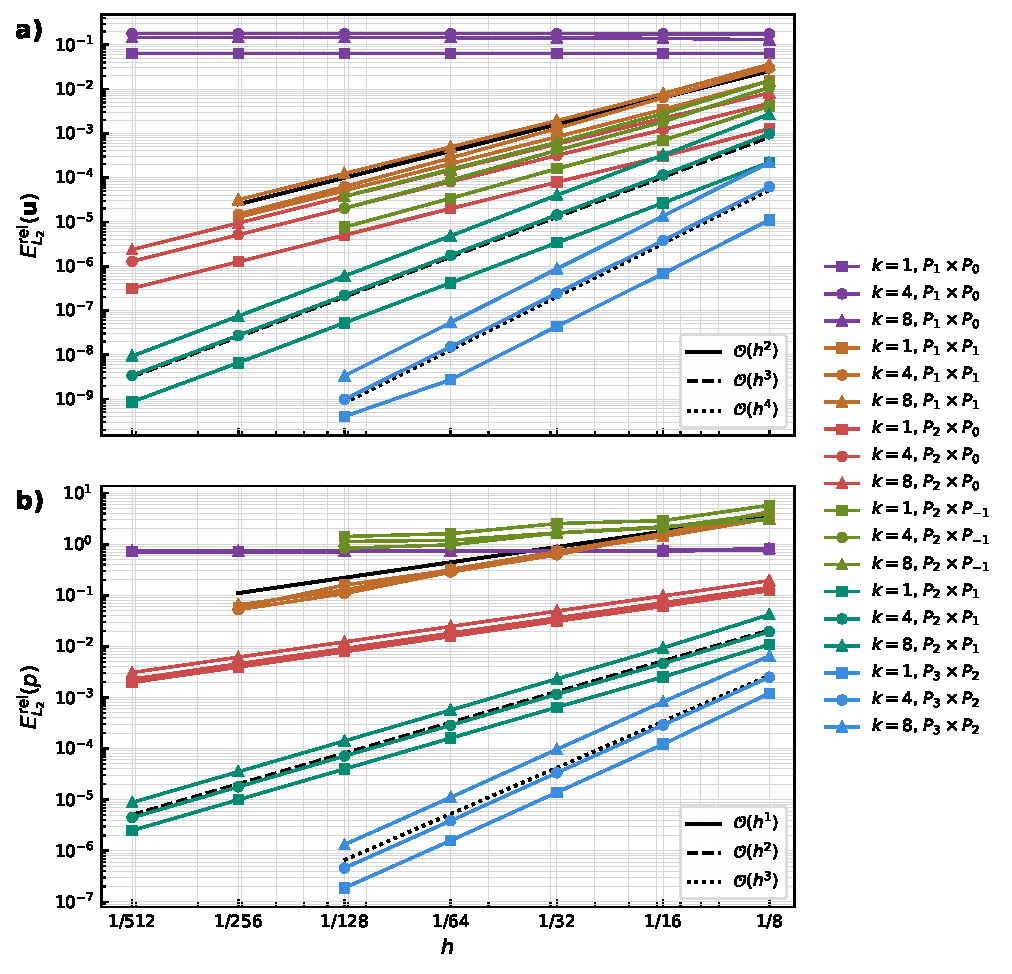
\includegraphics[width=0.95\linewidth,height=0.78\textheight,keepaspectratio]{Figures/figure_5_thieulot_annulus_convergence.pdf}
\caption{Velocity and pressure convergence for the Thieulot--Puckett annulus
benchmark.}
\label{fig:combined_thieulot_annulus_convergence}
\end{figure}

\begin{figure}[htb]
\centering
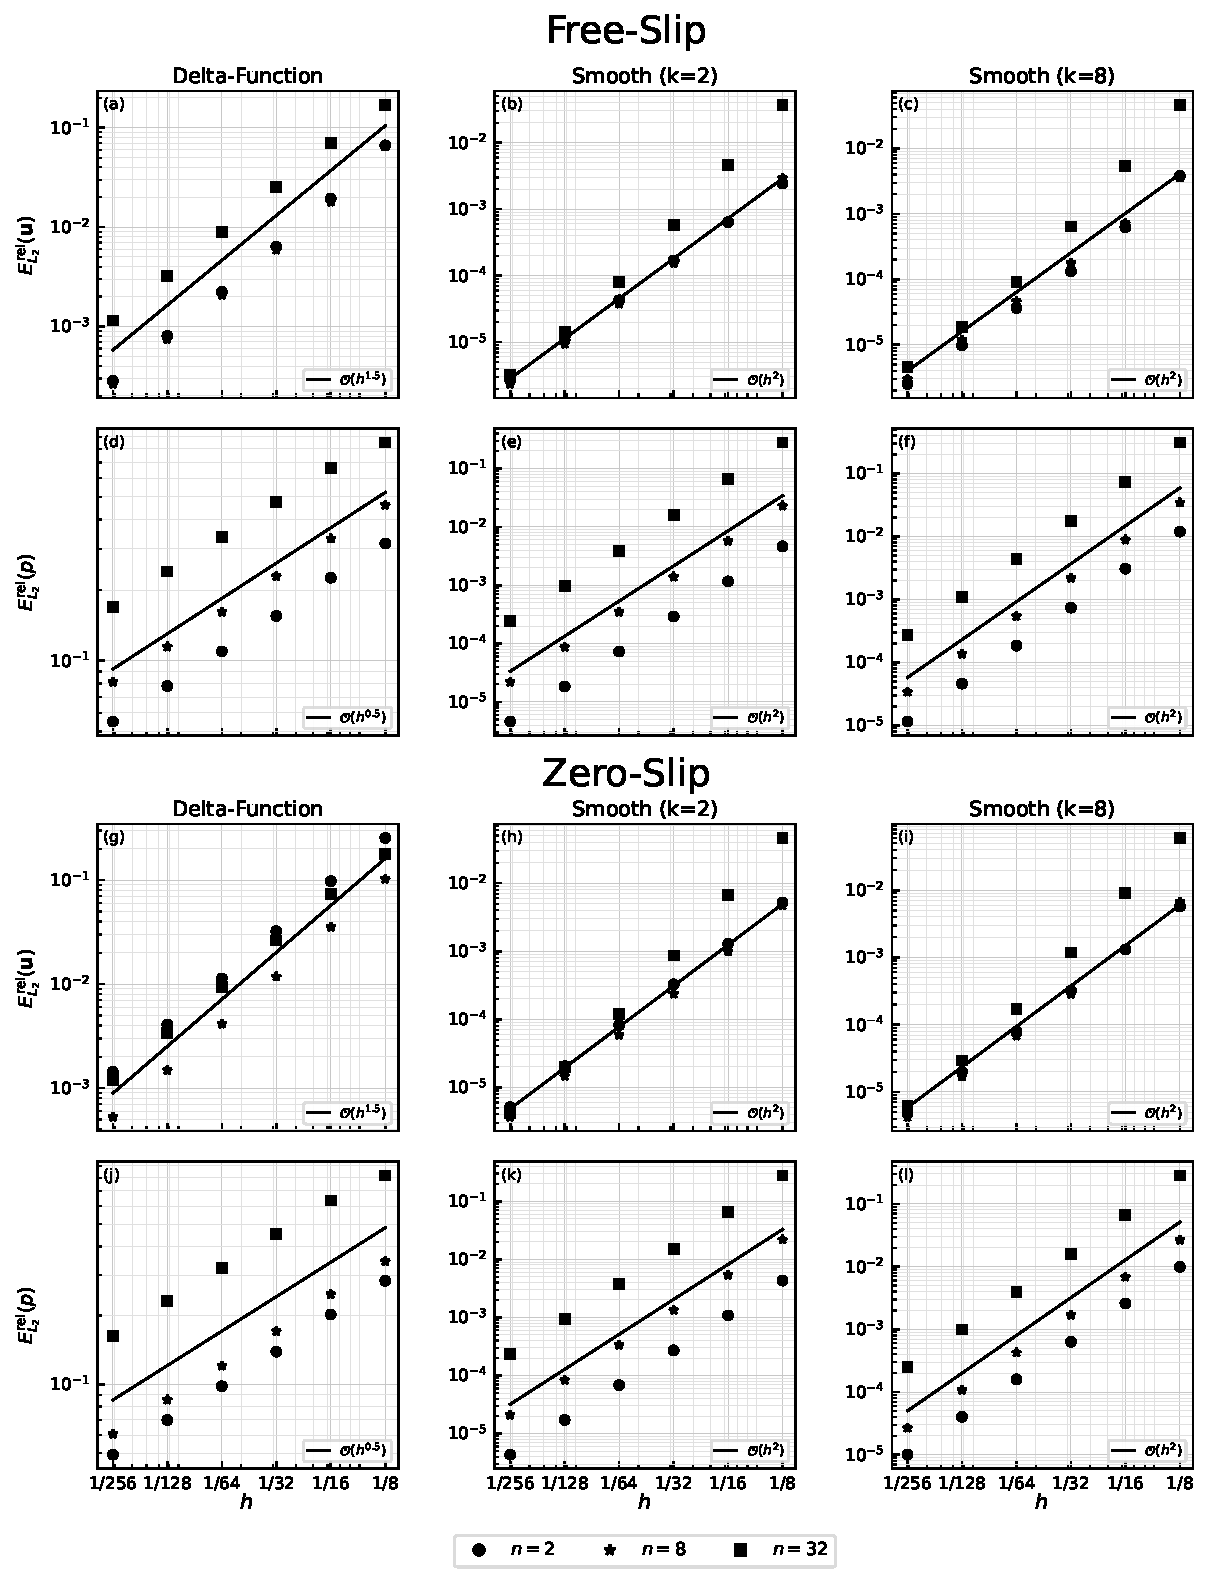
\includegraphics[width=0.95\linewidth,height=0.78\textheight,keepaspectratio]{Figures/figure_3_kramer_annulus_convergence.pdf}
\caption{Velocity and pressure convergence for the Kramer annulus benchmark.}
\label{fig:combined_kramer_annulus_convergence}
\end{figure}

\begin{figure}[htb]
\centering
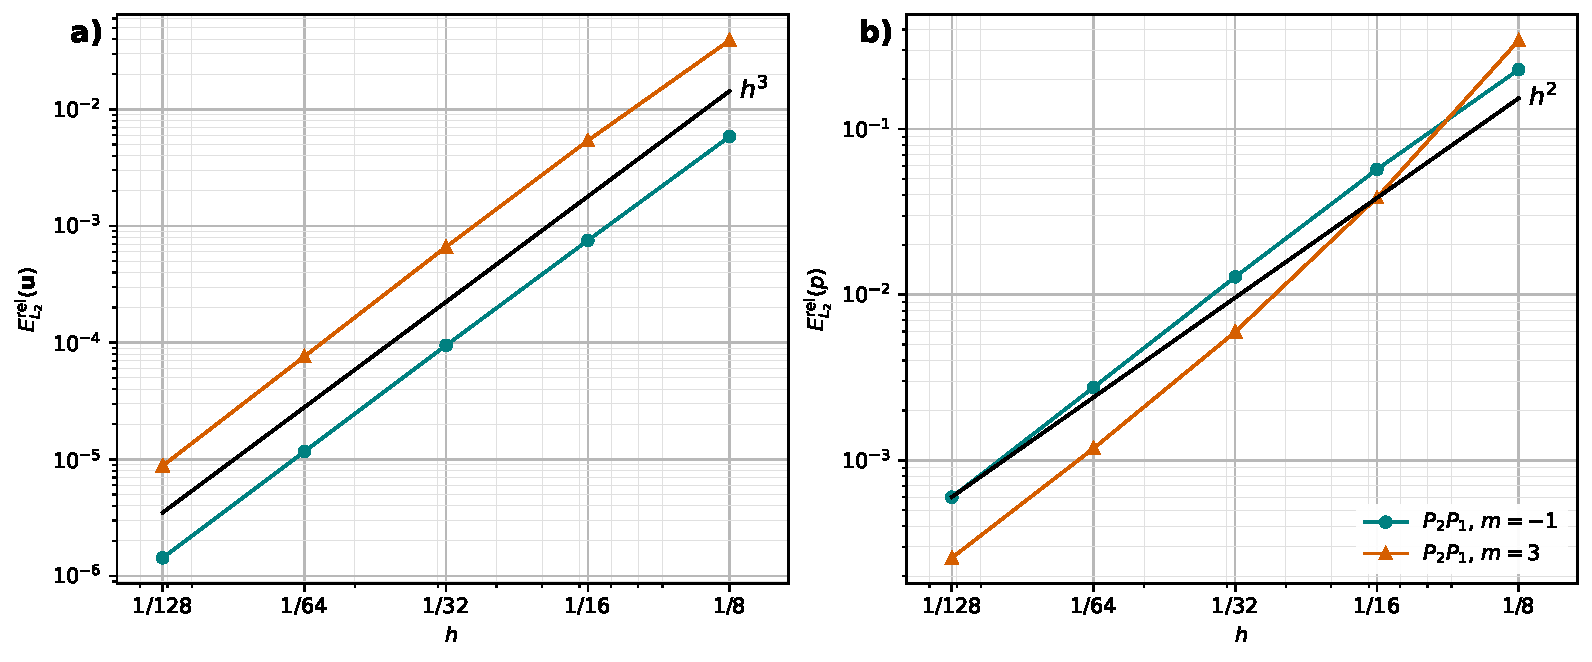
\includegraphics[width=0.95\linewidth,height=0.78\textheight,keepaspectratio]{Figures/figures_4_5_thieulot_convergence.pdf}
\caption{Velocity and pressure convergence for the Thieulot spherical-shell
benchmark.}
\label{fig:combined_thieulot_spherical_convergence}
\end{figure}

\begin{figure}[htb]
\centering
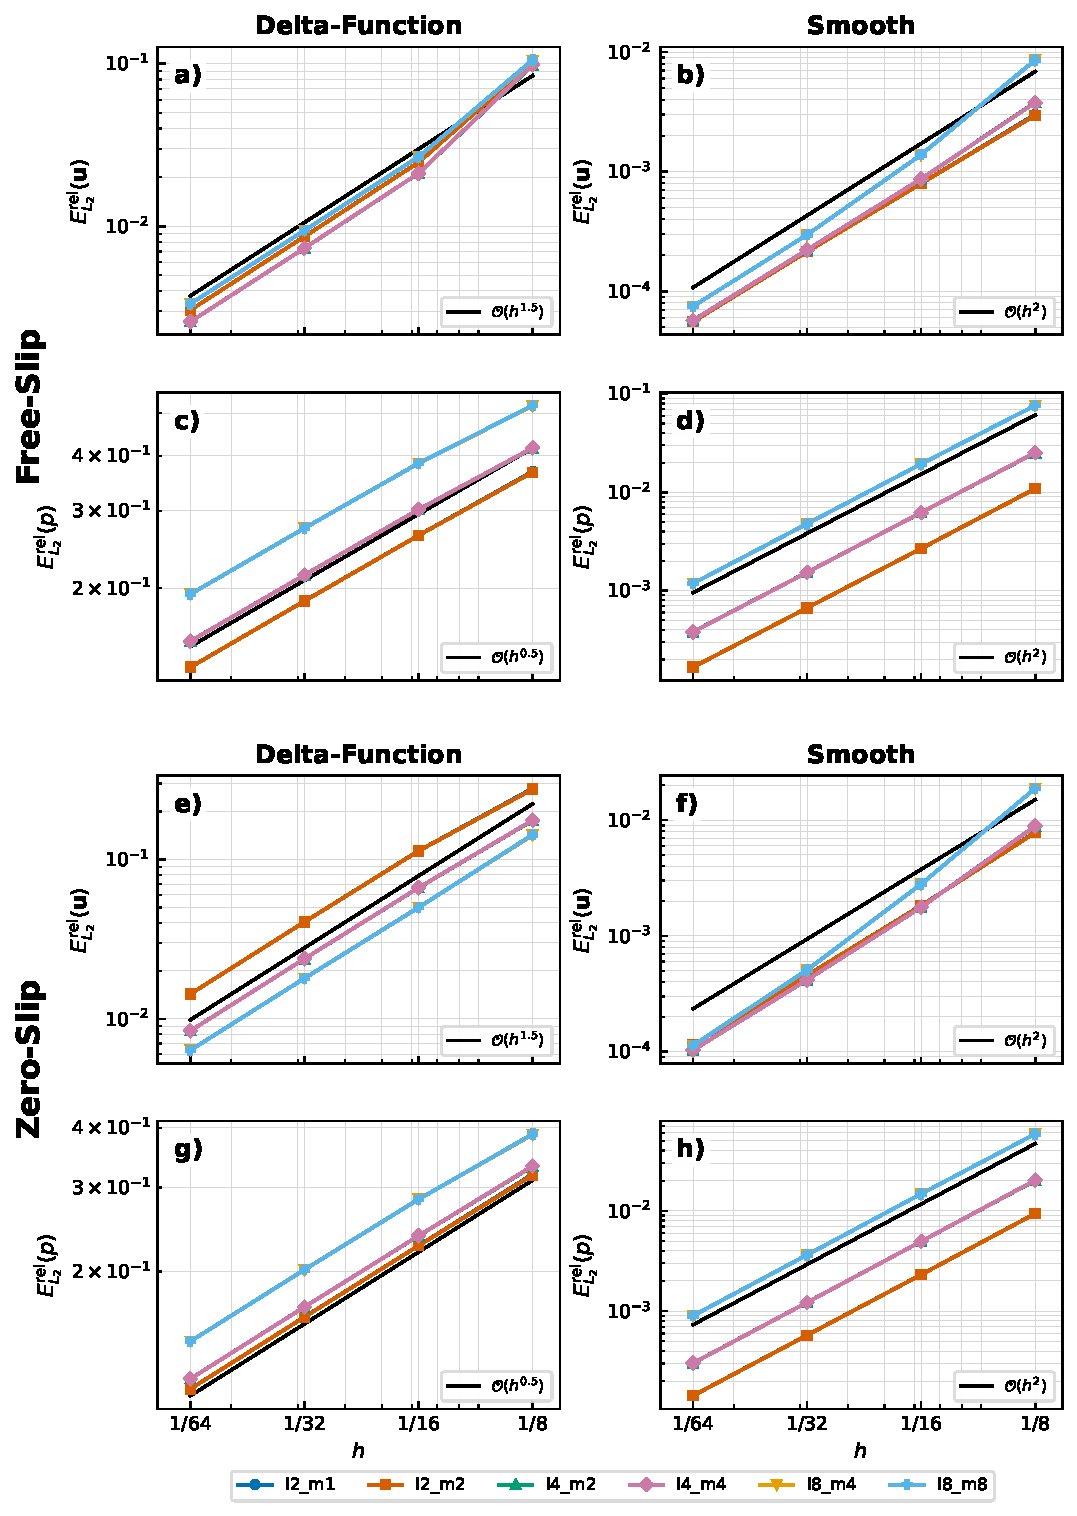
\includegraphics[width=0.95\linewidth,height=0.78\textheight,keepaspectratio]{Figures/figure_4_kramer_spherical_convergence.pdf}
\caption{Velocity and pressure convergence for the Kramer spherical-shell
benchmark.}
\label{fig:combined_kramer_spherical_convergence}
\end{figure}

\textbf{Results}
The smooth Thieulot--Puckett annulus benchmark reproduces the expected
convergence hierarchy for mixed finite-element discretisations. The
Taylor--Hood \(P_2\times P_1\) discretisation achieves approximately
third-order convergence in velocity and second-order convergence in pressure
in the volume \(L_2\) norm. Increasing the polynomial order to the
\(P_3\times P_2\) pair further improves the convergence rates to
approximately fourth order in velocity and third order in pressure before the
finest meshes begin to approach the numerical error floor. The
\(P_2\times P_0\) discretisation shows lower but still systematic convergence,
with velocity and pressure errors converging at approximately second and first
order, respectively.

For the Kramer annulus benchmark, the observed convergence behaviour depends
primarily on the regularity of the forcing term. The smooth volumetric forcing
cases recover close to the expected rates for the \(P_2\times P_1\)
discretisation, with pressure errors converging at approximately second order
and velocity errors showing second-order or better convergence. This behaviour
is consistent with the results reported by \citet{kramer2021}, where the use of
linear geometric meshes limits the velocity \(L_2\)-norm convergence to approximately
second order. Achieving the ideal third-order velocity convergence for the \(P_2\times P_1\)
discretisation requires a higher-order isoparametric approximation of the curved mesh
geometry. In contrast, the delta-function forcing cases introduce reduced solution regularity
through the internal interface, leading to slower convergence of approximately
\(O(h^{1.5})\) for velocity and \(O(h^{0.5})\) for pressure. These reduced
rates are expected from the analytical structure of the benchmark and do not
indicate a deficiency in the Stokes solver.

The three-dimensional Thieulot spherical-shell benchmark provides the clearest
smooth-solution verification case in spherical geometry. For the
\(P_2\times P_1\) Taylor--Hood discretisation, both the constant-viscosity and
radially varying viscosity models approach \(O(h^3)\) convergence in velocity
and \(O(h^2)\) convergence in pressure. These results confirm that the
spherical-shell Stokes implementation preserves the expected mixed
finite-element convergence hierarchy on curved three-dimensional domains.

The Kramer spherical-shell benchmark exhibits the same distinction between
smooth and singular forcing observed in the annulus configuration. The smooth
forcing cases produce pressure convergence close to \(O(h^2)\), while the
velocity errors converge at rates closer to \(O(h^2)\) than to the ideal
\(P_2\) \(L_2\)-norm rate over the tested mesh sequence. The delta-function
forcing cases again recover the expected reduced convergence trends of
approximately \(O(h^{1.5})\) in velocity and \(O(h^{0.5})\) in pressure.
Overall, the annulus and spherical-shell benchmark suites demonstrate that the
Stokes implementation reproduces the expected convergence behaviour for smooth
analytical solutions and the anticipated reduction in convergence rates when
the forcing contains singular internal interfaces.
